%%%%%%%%%%%%%%%%%%%%%%%%%%%%%%%%%%%%%%%%%%%%%%%%%%%%%%%%%%%%%%%%%%%%%%%%%%%%%%%
\chapter{Introduction} \label{ch:Introduction}
%%%%%%%%%%%%%%%%%%%%%%%%%%%%%%%%%%%%%%%%%%%%%%%%%%%%%%%%%%%%%%%%%%%%%%%%%%%%%%%

In this thesis we tell a story of how the theory of nonlinear waves shares a
deep connection with the field of algebraic geometry. In this chapter we
summarize this path, highlighting the primary objects at play.

% ------------------------------------------------------------------------------
\section{The Story} \label{sec:the-story}
% ------------------------------------------------------------------------------

The Kadomtsev--Petviashvili equation is a nonlinear partial differential
equation used to describe two-dimensional surface waves,
\begin{equation}
  \left( -4u_t + 6uu_x + u_{xxx} \right)_x + 3\sigma^2u_{yy} = 0.
\end{equation}
The KP equation is a generalization of the Korteweg-de Vries (KdV) equation,
\begin{equation}
  4u_t = 6uu_x + u_{xxx},
\end{equation}
and in fact the equation appears as a sub-expression in the KP equation. The
water waves modeled by the KP equation are typically of long wavelength and are
weakly two-dimensional in that there is a dominant direction of propagation with
smaller-scale oscillations ocurring in the transverse direction.

The KP equation admits a large family of quasi-periodic solutions of the form,
\begin{equation} \label{eq:finite-genus}
  u(x,y,t) = 2 \partial_x^2 \theta(z, \Omega),
  \quad
  z_j(x,y,t) = U_jx + V_jy + W_jt + \phi_j
\end{equation}
where $\theta : \mathbb{C}^g \times \mathbb{C}^{g \times g} \to \mathbb{C}$ is
the {\it Riemann theta function of genus $g$}. This space of solutions is dense
in the space of all periodic solutions and, therefore, fundamental to the study
of the equation.

\begin{figure}
  \centering
  \begin{subfigure}[b]{0.45\textwidth}
    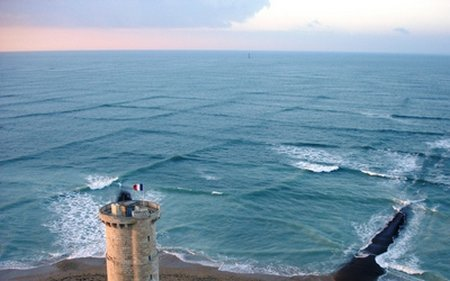
\includegraphics[width=\textwidth]{images/livekp.jpg}
    \caption{\^{I}le de R\'{e}, France}
    \label{fig:ile-de-re}
  \end{subfigure}

  \begin{subfigure}[b]{0.45\textwidth}
    \centering
    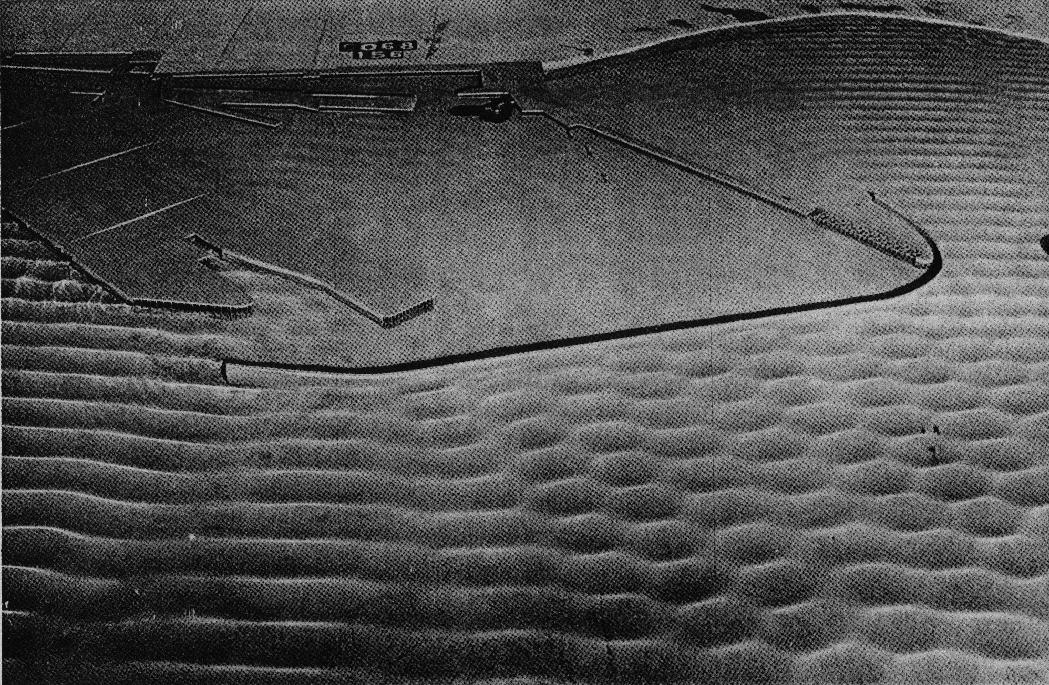
\includegraphics[width=\textwidth]{images/sd-harbor-model.jpg}
    \caption{Model of San Diego Harbor}
    \label{fig:san-diego-harbor}
  \end{subfigure}
  \label{fig:real-life}
\end{figure}

Before continuing with the story it is important to mention that KP-like waves
certainly appear in nature. In Figure \ref{fig:real-life} we see two examples of
the periodic structure emerging from chaotic conditions. The photograph in
Figure \ref{fig:ile-de-re} was captured on a particularly windy day off the
coast of \^{I}le de R\'{e} in France. Figure \ref{fig:san-diego-harbor} was
actually taken in the lab where a conference room-sized model of the proposed
San Diego harbor was constructed [TODO REF] before direct numerical simulation
was feasible. In this image we can see two phases of waves: on the bottom left
and top right there are long, KdV-like one-dimensional waves. In the bottom
right is the characteristic hexagonal wave structure of a ``typical'' KP
solution. We will later see that these structures correspond to different genera
of quasi-periodic KP solution.

Miraculously, the path to deriving and computing the finite-genus KP solutions
takes us through the field of algebraic geometry beginning in complex analysis
with algebraic curves. We give a brief glimpse into this path, here, and invite
the reader to examine the details in Chapter \ref{ch:2-background}. An algebraic
curve is the complex solution set to a bi-variate polynomial equation,
\begin{equation}
  C_f: \left\{
    (\lambda, \mu) \in \CC^2
    \; \big| \;
    f(\lambda, \mu) = 0, f \in \CC[x,y]
  \right\}.
\end{equation}
Algebraic curves are closely related to Riemann surfaces in that, modulo minor
details, a holomorphic mapping takes every algebraic curve to a Riemann surafce
and vice-versa.

Riemann surfaces are connected complex manifolds homeomorphic to a sphere with
$g$ handles (or a torus with $g$ holes) where $g$ is called the {\it genus}. One
can consider if there are any holomorphic one-forms defined on a given Riemann
surface and what kind of cycles (simple closed paths) they could be integrated
on. It turns out that the space of holomorphic one-forms is $g$-dimensional and
the space of homologous paths is $2g$-dimensional. Lets label the bases elements
of these spaces $\{\omega_1, \ldots, \omega_g\}$ and $\{ a_1, \ldots, a_g,
b_1, \ldots, b_g\}$, respectively. Naturally, we can then determine the $2g^2$
resulting integrals, or {\it periods},
\begin{equation}
  A_{ij} = \oint_{a_j} \omega_i, \quad B_{ij} = \oint_{b_j} \omega_i.
\end{equation}
These two quanties together form the {\it period matrix} of the Riemann surface
/ algebraic curve. After normalizing the holomorphic one-forms such that $A_{ij}
= \delta_{ij}$, the Kronecker delta function, we obtain the period matrix $\tau
= [I; \Omega]$. The quantity $\Omega$ appears in the finite-genus solutions
given in Equation \ref{eq:finite-genus}, above.

The other parameters, $U, V, W, \phi \in \mathbb{C}^g$ are also determined from
the Riemann surface from a specified collection of {\it places} on the Riemann
surface also called a {\it divisor}. The parameters themselves are computed by
evaluating two functions, the Abel map and the Riemann constant vector, at the
pdivisor. In particular, this divisor encodes information about the initial
condition of the desired finite-genus solution if one were solving the KP
initial value problem.

Finally, this mathematical path from algebraic curves to KP solutions can be
made extraordinarily concrete: each step outlined above can be computationally
realized. As Field's Medalist William Thurston recognizes, without attention to
detial this is a challenging feat. By developing algorithms along the way we
accomplish two things. First, we provide an experimental tool for the study of
periodic KP waves. Second, and more importantly, with the use of sound software
design principles we create a general framework for performing analytic
calculations on Riemann surfaces that both is computationally efficient and is
easily extendible by future researchers. The development of such a framework
extends the reach of the code to beyond the application to non-linear waves and
serves the mathematical community.

% ------------------------------------------------------------------------------
\section{Outline} \label{sec:outline}
% ------------------------------------------------------------------------------

Chapter \ref{ch:background} presents a succinct introduction to the field of
complex algebraic geometry and Riemann surfaces. A student approaching the
subject need only the basics of complex analysis to get started. It begins with
an introduction to algebraic curves and their geometry. We then connect these
curves to the theory of Riemann surfaces and demonstrate, at least in the
compact and connected case, that the two are synonymous. The bulk of the chapter
dives deep into the study of Riemann surfaces from this perspective of algebraic
curves building up the necessary machinery needed to define the {\it Jacobian}
of a Riemann surface and its associated {\it Period Matrix}; central objects of
focus for much of the work in this thesis as well as current research in the
field. The chapter concludes with two key objects defined on the Jacobian, the
{\it Abel Map} and {\it Riemann Constant Vector}, as well the {\it Riemann theta
  function}. Each of these are primary ingredients in the connection to and
calculation of solutions to the Kadomtsev-Petviashvili equation.

If Chapter \ref{ch:background} presents the theory then Chapter
\ref{ch:abelfunctions} contains the corresponding algorithms which allow us to
experiment with Riemann surfaces on a computer. For each key concept described
in the previous chapter we present efficient algorithms for their computation
along with a collection of examples. These algorithms are gathered together in a
Sage package called {\it Abelfunctions}. We spend some time in this chapter
discussing the high-level design of this package including how important
principles in software design allows the package to be easily extendible.

Chapters \ref{ch:kp} and \ref{ch:determinantal} showcase the use of these
algorithms to compute the finite-genus solutions to the Kadomtsev-Petviashvili
equation as well as determinantal representation of algebraic curves. Previous
approaches to computing periodic solutions to KP are either too restrictive (the
resulting solution space is not dense in the space of periodic solutions) or
rely on direct numerical simulation where the accuracy of the solution degrades
over time. In contrast, the finite-genus solutions derived by the Riemann
surface machinery is valid for all space and time. The work on determinantal
representations presented here is the computational realization of the theory
developed by Helton and Vinnikov, the importance of which lies in the
application to polynomial optimization algorithms.

% ------------------------------------------------------------------------------
\section{Acknowledgements} \label{sec:acknowledgments}
% ------------------------------------------------------------------------------

First and foremost I would like to thank my wife, Megan Karalus. Thank you for
your love and unending patience. You stood by me when things got tough,
celebrated with me when things got better, and encouraged me to finish what I
started. Thank you to the many people in the Applied Mathematics department at
the Univeristy of Washington for shaping me into the mathematican, computer
scientist, and human being that I am today. Bernard for his mentorship and
comraderie, Randy for encouraging me to keep one toe in the HPSC world, Lauren
for her friendship and counsel; and Daniel, Lowell, and Alan for their
friendship and the many hours spent at the College Inn. Thank you to Amazon AI
for believing that I can make a difference in this world by creating great
things and by providing a rich an supportive environment where the interface
between mathematical research and high performance computation find a natural
home. Finally, this work was generously supported bpy the National Science
Foundation under grant NSF-DMS-1008001. Any opinions, findings, and conclusions
or recommendations expressed in this material are those of the authors and do
not necessarily reflect the views of the funding sources.
